I collected two different types of data for 143 dispute cases 
requested to the WTO DSB
\footnote{List of collected case numbers are 
available at \hyperref[sub:cited-articles-table]{Appendix A.3}
}.
One is textual description of trade policy 
that led to the dispute \hyperref[sub:factual-aspect-example]{(Appendix A.2)} and the other one is 
set of articles of the WTO agreement that are
cited for each dispute \hyperref[sub:cited-articles-table]{(Appendix A.3)}. 
I will explain the format and the content of 
each type of data with an example. 
% Technical details about the automated way 
% of collecting data will be
% explained in the \hyperref[appendix:panel-report-toc]{Appendix A.4}.

\begin{figure}[h]
    \centering
    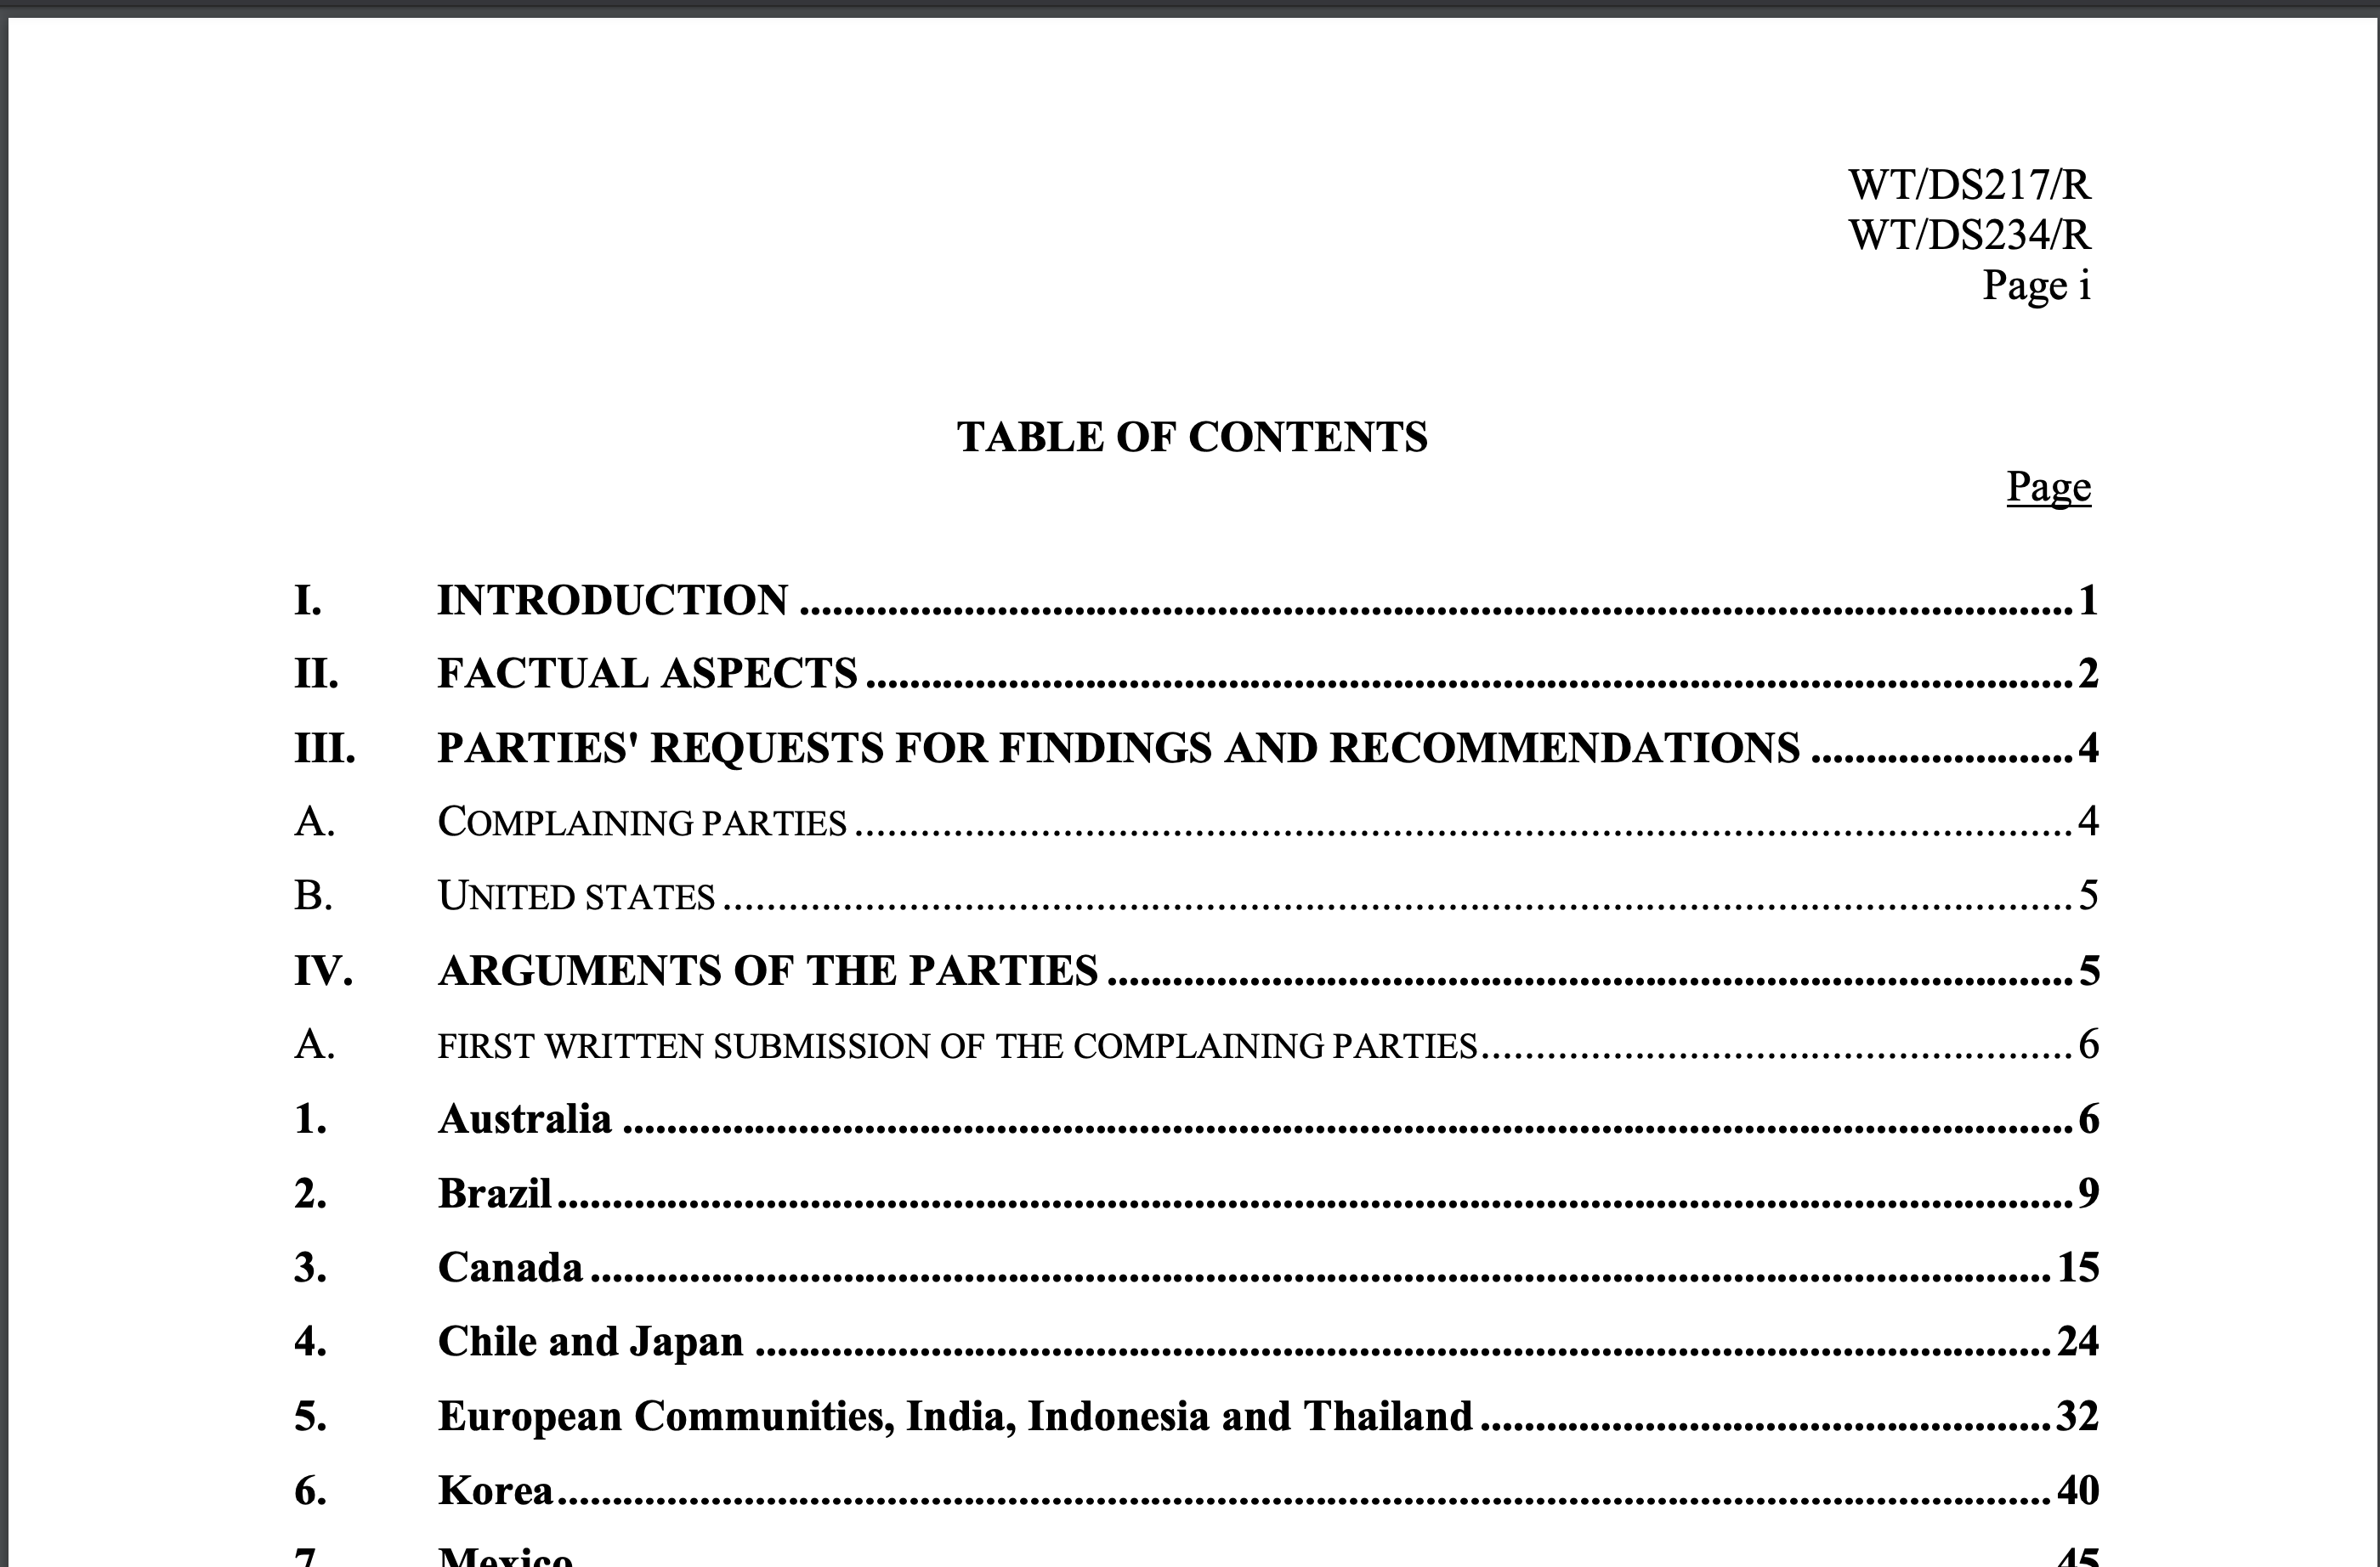
\includegraphics[scale=0.28]{Data/pngs/panel_report_toc.png}
    \caption{
        {\bf Table of Contents of Panel Report: }Panel provides 
        factual aspect in the panel report with its page location.
        }
    \label{fig:panel-report-toc}
\end{figure}
% \begin{center}
%     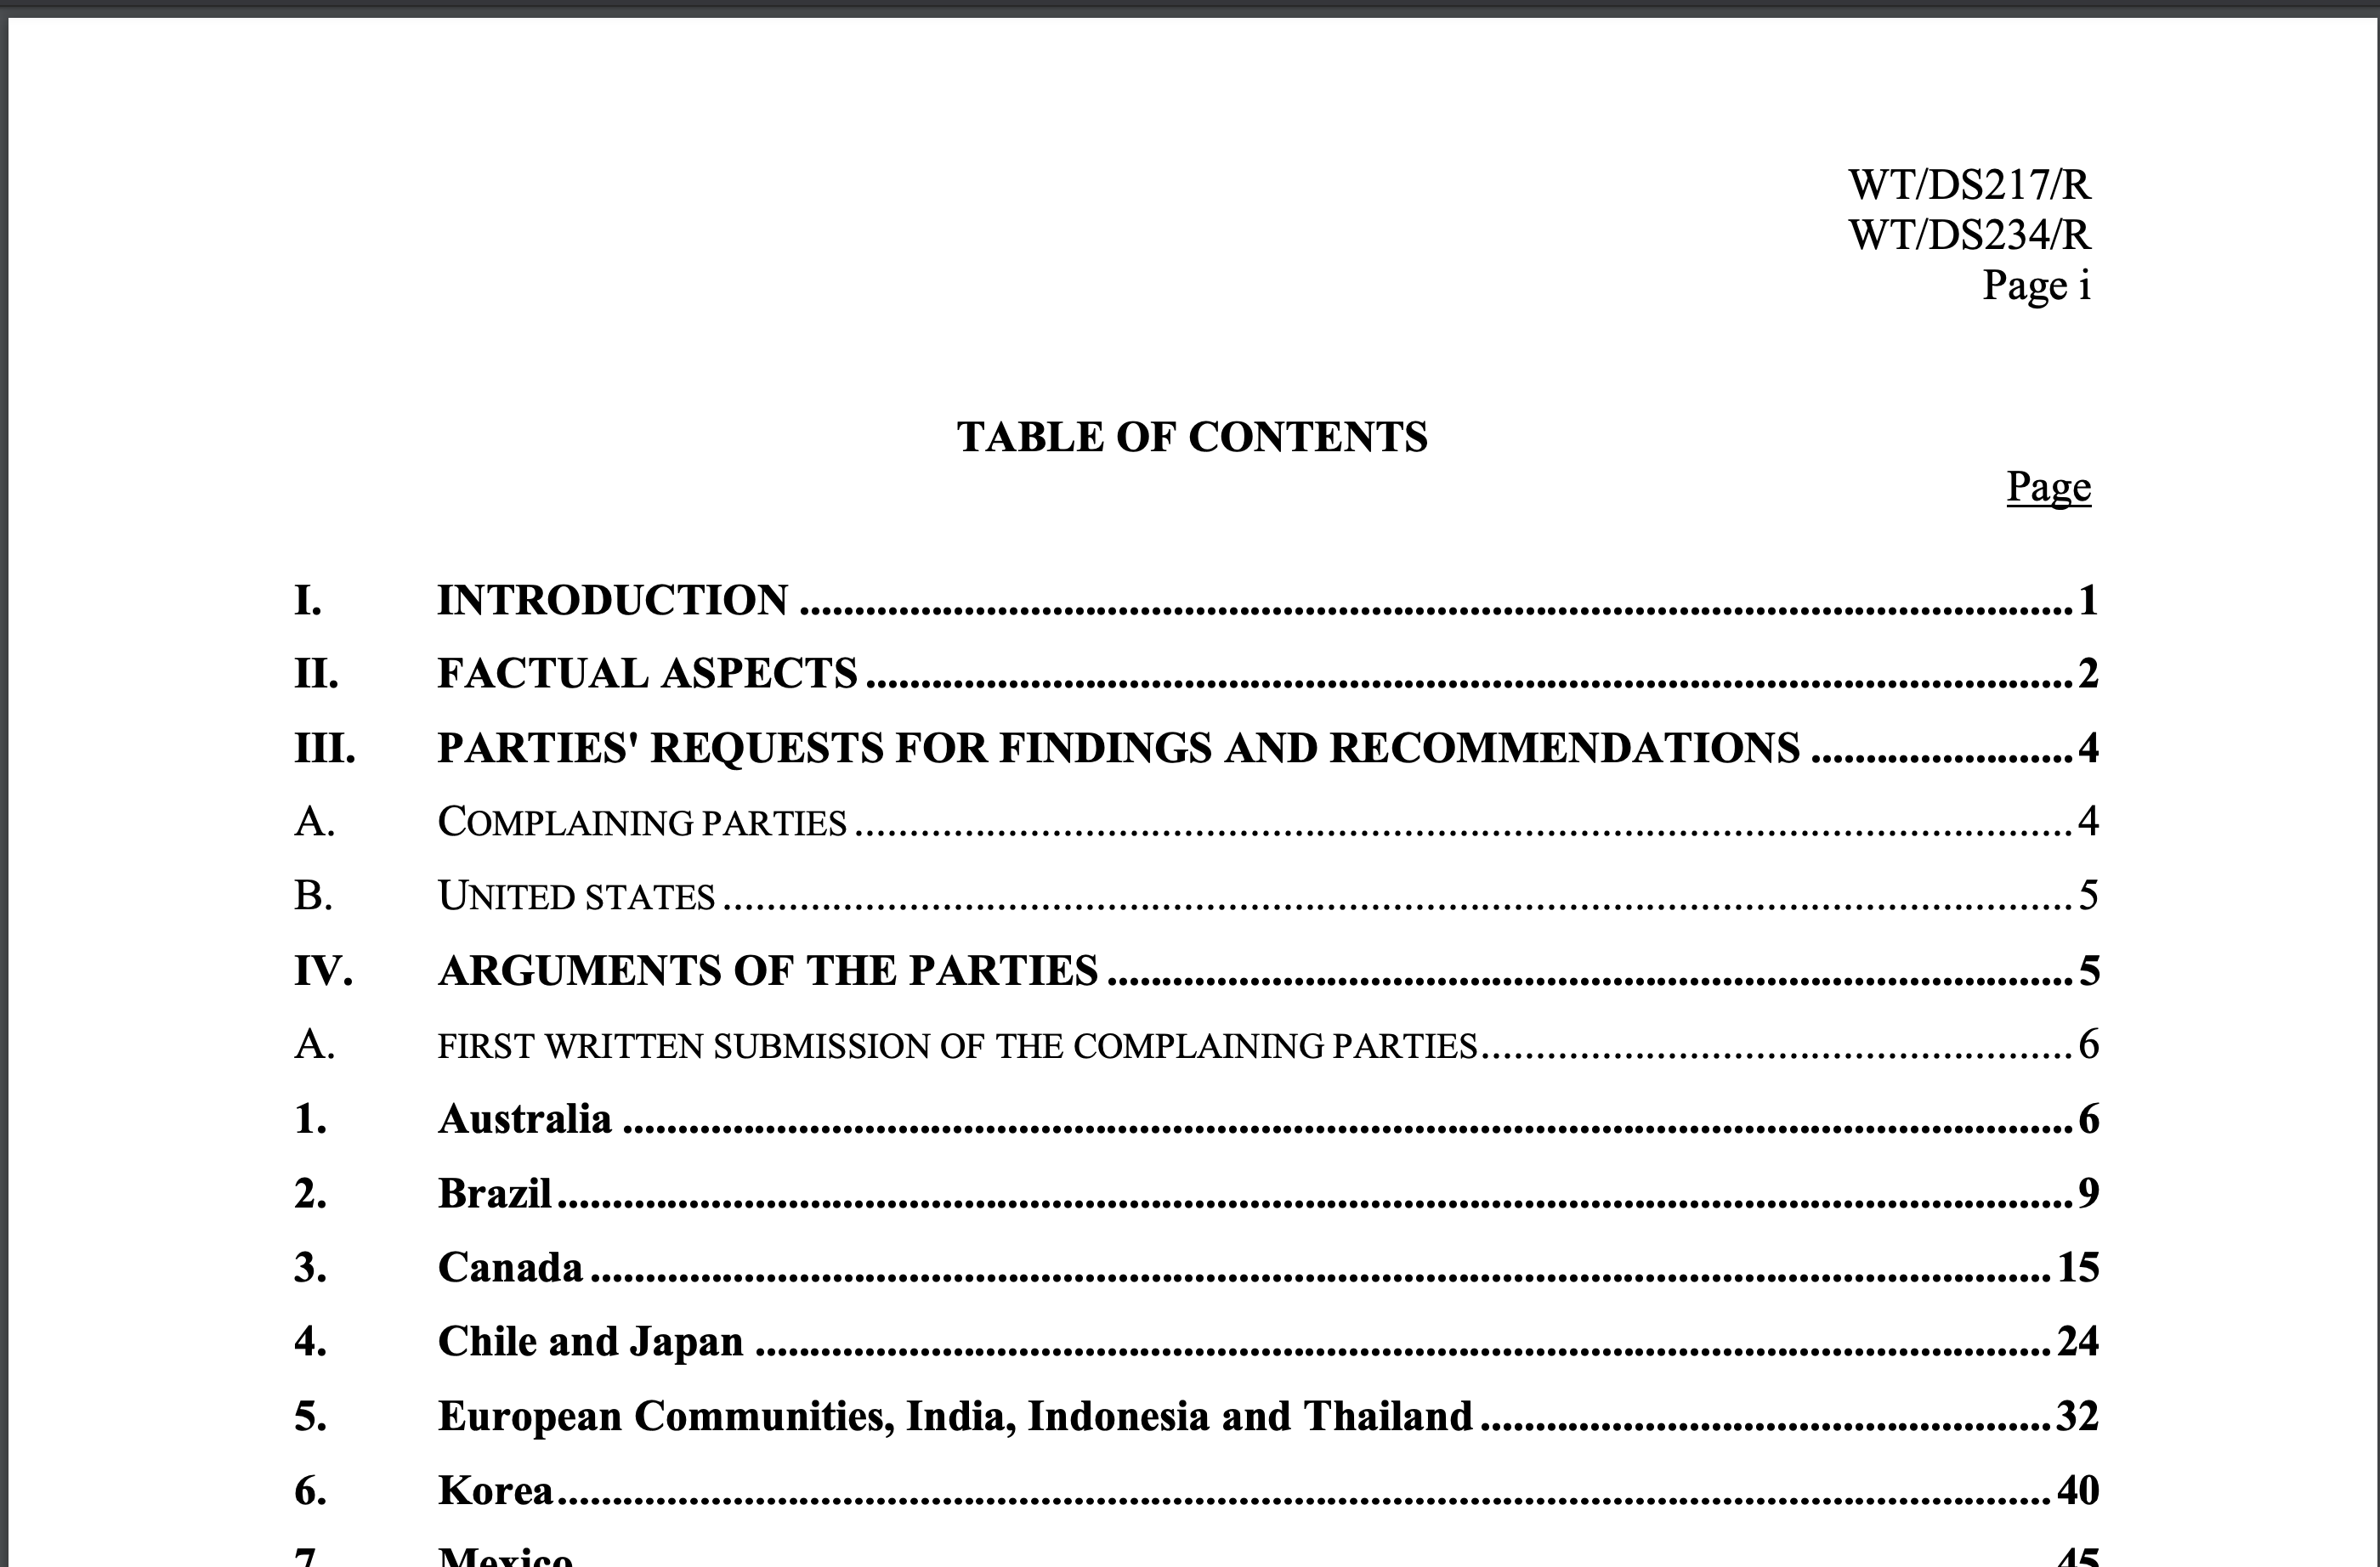
\includegraphics[scale=0.3]{Data/pngs/panel_report_toc.png}
% \end{center}


% This section explains how I collected 
% which data to train the neural network. 
% Basically, 





% I collected two different 
% types of data, one is textual description of trade policy 
% that led to the dispute and the other one is 
% set of articles of the WTO agreement that are
% cited for the dispute.s



% \begin{displayquote}
%     ``Korea' s domestic support for beef in 1997 and 1998 exceeded the de minimis level contrary to Article 6 of the Agreement on Agriculture.''
%   \end{displayquote}
  
%   \begin{itemize}
%     \item exemplify as detail as possible to inform readers about how data looks like.
%     \item Privide a running example that shows how WTO works with data. 
%     \item (Borrow from the previous paper)
    
%   \end{itemize}
  